\documentclass[a4paper,11pt]{article}
\usepackage[utf8]{inputenc}
\usepackage[francais]{babel}
\usepackage{graphicx}
\usepackage{fancyhdr}
\usepackage {color}
\usepackage{colortbl}
\usepackage{hyperref}
\usepackage{listings}

% Title Page
\title{SPAM ASSASSIN}
\date{Décembre 2014}
\author{Mathieu KERN - Aymeric HINDERCHIETTE}
\pagestyle{fancy}


\begin{document}

\maketitle
\includegraphics{spamassassinintro.png}
\pagebreak

\tableofcontents

\pagebreak

\part{Présentation de SpamAssassin}

\section{Problématique }

  Le mail (ou courriel) est aujourd'hui le moyen privilégié de communication à travers le monde. Massivement utilisé, 
d'une certaine fiabilité et éprouvé par des décennies d'utilisation il reste le moyen le plus répandu pour 
les communications entres les personnes. Malheureusement, mail est également aujourd'hui synonyme de spam, ces messages
indésirables qui s'entassent dans nos boites mails. C'est ici qu'entre en jeu SpamAssassin.

\subsection{Le SPAM}
Avant de poursuivre sur SpamAssassin, rappelons concrètement ce qu'est le SPAM et ce qu'il implique. 

\paragraph{Comment reconnaître un SPAM:}

\begin{itemize}
 \item De par sa nature, un SPAM n'est pas désiré par l'utilisateur qui le reçoit. 
 \item La réception d'un SPAM résulte d'un envoi massif: une machine (souvent un bot) envoie le même message 
 à plusieurs destinataires sans aucun discernement. Cela s'oppose aux messages ciblés par exemple de commerçant,
 qui n’envoie que à leurs prospects (à but publicitaire ou informatif).
 \item Son contenu n'est pas destiné spécifiquement à l'utilisateur (chaque personne reçoit le même contenu).
 \item Une importante liste de destinataires.
 \item Entête des messages souvent corrompues ou ne respectant pas les normes.
\end{itemize}

\paragraph{Statut légal}


La loi pour la confiance dans l'économie numérique du 21 juin 2004 contient une transposition de la
directive européenne du 12 juillet 2002\footnote{Le principe introduit figurera également à l'article L.34.5 du code 
des postes et des communications électroniques } relative à la protection de la vie privée dans le secteur des communications
électroniques:
\begin{quote}
 Est interdite la prospection directe au moyen d'un automate d'appel, d'un télécopieur ou d'un courrier électronique utilisant,
 sous quelque forme que ce soit, les coordonnées d'une personne physique qui n'a pas exprimé son consentement préalable à recevoir
 des prospections directes par ce moyen. 
\end{quote}
Les SPAM sont donc connus du droit français et encadrés par des textes spécifiques.

\section{Le projet}

\subsection{Informations}


\begin{center}
\begin{tabular}{cll}
\hline
Développeur & Apache Software Foundation  \\
Langage & Perl 
Dernière version & 3.4.0 (11 février 2014) [+/-] \\
Environnements & Multiplate-forme  \\
Type & Anti-spam & \\
Licence & Licence Apache 2.0 \\ \\
\hline
\end{tabular}
\end{center}



SpamAsassin est donc aujourd'hui sous le giron de la Apache Software Foundation, organisation à but non lucratif qui
s'occupe également du serveur Apache, Logiciel de distribution de contenu WEB le plus utilisés au monde. 
Elle gère également 150 autres projets.
EN outre tout ses projets sont distribués sous sa propre Licence, la licence Apache(actuellement en 2.0) , qui est compatible GPL v3.
Cette licence met l’accent sur le copyright tout en restant bien sur une licence libre. Les objectifs principaux de la Fondation sont de protéger 
juridiquement le travail des contributeurs et d'empêcher que la marque Apache soit utilisée illégalement.

Le projet SpamAssassin est actif depuis plus d'une décennie et est constamment en développement 
pour s'adapter aux développements des méthodes qu'utilisent les spammeurs. C'est en outre le programme anti-spam le plus utilisé à cause de son efficacité.

\subsection{Développement}

SpamAssasin contient environ 300 000 lignes de codes ce qui en fait un très gros projet( Graphique ~\ref{fig:code}).
Le projet est à maturité et il ne grossit plus depuis plusieurs années, les développeurs se concentrant sur l'optimisation du code existant.
Il y actuellement 23 développeurs pricnipaux, avec une répartition des lignes codes assez inégales, notamment deux développeurs qui ont fait la majorité du code( Tableau ~\ref{tab:devs}).
Mais vu que c'est un projet libre et open source, chacun est libre de contribuer et forker le projet. Cela concerne aussi 
bien les particuliers que les entreprises (En respectant bien sur les restirction de la licence Apache).

\begin{figure}
 \includegraphics[width=\textwidth]{annexes/lignes.png}
  \caption{Évolution du nombre de ligne de codes}
  \label {fig:code}
\end{figure}

\begin{table}
 
\definecolor{tcA}{rgb}{0.627451,0.627451,0.643137}
\begin{center}
\begin{tabular}{lllll}

\rowcolor{tcA}
 Author Id & Changes & Lines of Code & Lines per Change\\
\rowcolor{tcA}
 Totals & 26092 (100.0\%) & 1403447 (100.0\%) & 53.7\\
\rowcolor{tcA}
  jm & 8136 (31.2\%) & 721593 (51.4\%) & 88.6\\
\rowcolor{tcA}
  spamassassin role & 7997 (30.6\%) & 463448 (33.0\%) & 57.9\\
\rowcolor{tcA}
  axb & 741 (2.8\%) & 54525 (3.9\%) & 73.5\\
\rowcolor{tcA}
  mmartinec & 1779 (6.8\%) & 32348 (2.3\%) & 18.1\\
\rowcolor{tcA}
  felicity & 1625 (6.2\%) & 29134 (2.1\%) & 17.9\\
\rowcolor{tcA}
  kmcgrail & 605 (2.3\%) & 21294 (1.5\%) & 35.1\\
\rowcolor{tcA}
  quinlan & 1100 (4.2\%) & 19583 (1.4\%) & 17.8\\
\rowcolor{tcA}
  parker & 309 (1.2\%) & 10407 (0.7\%) & 33.6\\
\rowcolor{tcA}
  khopesh & 1369 (5.2\%) & 10296 (0.7\%) & 7.5\\
\rowcolor{tcA}
  dos & 427 (1.6\%) & 8427 (0.6\%) & 19.7\\
\rowcolor{tcA}
  jhardin & 1021 (3.9) & 6845 (0.5\%) & 6.7\\
\rowcolor{tcA}
  wtogami & 137 (0.5\%) & 6470 (0.5\%) & 47.2\\
\rowcolor{tcA}
  hstern & 63 (0.2\%) & 6029 (0.4\%) & 95.6\\
\rowcolor{tcA}
  sidney & 275 (1.1\%) & 3552 (0.3\%) & 12.9\\
\rowcolor{tcA}
  jquinn & 28 (0.1\%) & 2181 (0.2\%) & 77.8\\
\rowcolor{tcA}
  mss & 133 (0.5\%) & 2072 (0.1\%) & 15.5\\
\rowcolor{tcA}
 hege & 95 (0.4\%) & 1931 (0.1\%) & 20.3\\
\rowcolor{tcA}
 duncf & 109 (0.4\%) & 1892 (0.1\%) & 17.3\\
\rowcolor{tcA}
  jgmyers & 66 (0.3\%) & 508 (0.0\%) & 7.6\\
\rowcolor{tcA}
  smf & 35 (0.1\%) & 499 (0.0\%) & 14.2\\
\rowcolor{tcA}
  maddoc & 11 (0.0\%) & 319 (0.0\%) & 29.0\\
\rowcolor{tcA}
  fanf & 12 (0.0\%) & 49 (0.0\%) & 4.0\\
\rowcolor{tcA}
  kb & 19 (0.1\%) & 45 (0.0\%) & 2.3
\end{tabular}
\caption{Statistique des développeurs du projets }
\footnotesize{Source \footnote{Tableau généré avec StatSVN à partir des sources de SpamAssassin}}
\label{tab:devs}
\end{center}
\end{table}


\subsection{Qu'est ce que SpamAssassin}

SpamAssassin est un programme écrit en PERL dont le but est de filtrer activement les Emails en se basant sur des mécanismes internes. 
SpamAssassin n'effectue aucune action envers les mails, il ajoute seulement des informations personnalisés
qui peuvent être utilisée par d'autres programmes pour effectuer des actions sur les mails (les ranger des dossiers distincts, les supprimer, les bloquer, \dots)


Il peut être utilisé de plusieurs manières:
\begin{itemize}
 \item En mode client, lancé à chaque fois que l'on fait appel à lui
 \item En mode demon grâce à \emph{spamd} , les appels au demon étant fait avec l'utilitaire \emph{spamc}.
 \item Comme une interface de programation: des programmes qui nécessitent des fonctionnalités de filtrage de SPAM peuvent s'interfacer avec SpamAssin
 pour construire des solutions utilisant ses fonctionnalités
\end{itemize}

\pagebreak

\part{Ses fonctionnalités}

\section{Comment il filtre}

SpamAssassin reçoit des mails que lui redirigent d'autres programmes, y effectue des tests pour déterminer si ce sont des SPAMS, 
puis renvoie les mails testés au programme qui les as envoyés.

\subsection{Les test de SpamAssassin }

\begin{description}
 \item [Champs d'entête] En se basant sur la forme des entêtes et en les comparant avec des schéma connus par SpamAssasin. En effet 
 on peut se base sur la façon dont certains systèmes de SPAMs construisent leurs messages pour les filtrer. 
 \item [Corps du message] Bien sur SpamAssasin permet de filtrer les mails suivant les mots et expressions qu'ils contiennent. 
 ``ceci n'est pas un SPAM'', ``Bonjour jes suis une princesse d'un royaume africain'', ``Venez chechez votre lot'', \dots sont des expressions
 typiques pour des SPAMs. 
 \item [Filtre bayésien(détail plus loin ~\ref{baye})] Filtrer les entêtes et le corps d'un message résultera toujours en de multiples faux positifs. C'est ici que le filtrage 
 bayésien se révèle interessant car il va prendre en considération ce que l'on considère comme SPam et non SPAM soit des ``bon mails'' (``HAM'' en anglais).
 Il va ensuite utiliser les repertoires de SPAMs connu et de ``HAM``  connus, pour y identifier les mots et phrases (Définits comme ''Tokens`` en anglais)
 qui n'apparaissent que dans les SPAMs et que dans les ''HAMs``.
 Un token SPAM trouvé resultant d'une hausse du score (voir \ref{score}) SPAM, un token résultant en une baisse de ce niveau. Ce filtrage permet d'être plus précis et d'éviter les faux positifs, 
 en ne se basant pas juste sur un mot ou une phrase mais des ensembles. 
 \item [List noire/blanche automatique] SpamAssassin garde automatiquement une liste blanches des expéditeurs des mails.
 Pour chaque nouveau mail le programme compare le mail précédent provenant de la même adfresse mail et adresse IP.
 Comme précédemment si une adresse email a envoyé un SPAM, ce nouveau mail verra son score abaissé. A l'inverse si c'était un bon mail son score 
 se verra baisser.
 \item [Liste noire/blanche manuelle] Il est tout à fait possible de définir ses propres listes, en autorisant ou 
 interdisant des mails de certaines adresses
 \item [Signalements] En utilisant des signatures établis à partir de mails signalés par les utilisateurs. Il y a notamment les projets DCC, Pyzor, et Razor2
 qui possèdent des bases de données de mails signalés comme SPAM. SpamAssassin va ainsi demander à ces bases si les mails qu'il reçoit 
 sont présents dans leurs donnée.
 \item [DNS blocklists] Ce sont des des bases de données contenant des adresses IP signalées comme expédiant du SPAM ou mal 
 configurée(Par exemple en étant un relais ouvert). Également sont pris en compte les IP de particuliers (considérant qu'il y a peu de chance
qu'un particulier envois directement des mails sans passer par son FAI. Ces signalements vont être pris en compte par SpamAsassin pour le score des mails.
Il intègre nativement quelque une de ces listes.
\item [Caractères et langues] on peut spécifier des caractères et langues comme SPAM.

C'est ces ensembles de règles qui fonctionnant conjointement permettent à SpamAssassin de garantir un haut 
niveau de fiabilité de détection des SPAM, un test pouvant ne pas fonctionner mais sera contrebalancé par les autres.
 \end{description} 


Spam Assassin effectue sur chaque mail qui lui est donné à traiter une série de test, qui vont ensuite donner lieu à un score, qui sera indiqué dans un entête 
si il est considéré comme SPAM. 
Ce résultat sera ensuite utilisé par d'autres programmes pour déterminer des actions à entreprendre.


\section{Le score} \label{score}
C'est la base du signalement des SPAM de SpamAsassin. Un mail après avoir subi des test différents se voit attribuer une note. Cette note permet
ensuite de définir des actions à effectue. Quand un mail est considéré comme SPAM, SpamAssassin ajoute ses propres entêtes (Exemple ~\ref{fig:ex_score}):
\begin{itemize}
 \item ''-Spam-Level: \*\*\*\*\*\*\*\*\* '': Renseigne le score (ici 9)
 \item -Spam-Status: Yes, score=9.0 required=5.0 tests=BAYES\_99,FROM\_EXCESS\_BASE64,FR\_HOWTOUNSUBSCRIBE,FR\_SPAMISLEGAL \dots : Indique des informations relatives aux test effectués et la configuration)
\end{itemize}

. L'utilisateur peut paramétrer ce score pour définir une marge de définitions des SPAMs(valeurs ''require``). Une fois ce score ateint le mail est considéré comme SPAM.
C'est ensuite aux autres programmes d'utiliser ces données. Par exemple on pourrait configurer un MUA pour qu'il sépare 
les SPAM par score suivant des filtres définit. 

\label{baye}
\section{Le filtre bayésien}


Une fonctionnalité qui est une des plus importantes caractérsitiques de SpamAssassin est sans doute son filtre
bayésien\footnote{\href {https://fr.wikipedia.org/wiki/Th\%C3\%A9or\%C3\%A8me\_de_Bayes}{Théorème de Bayes}}.
Il va permettre d'établir une connaissance des éléments qui constituent un SPAM et ceux qui n'en sont pas.
\paragraph{Uilisation par SpamAssassin}

Comme ennoncé plus haut, ce type de filtre fait partis de son arsenal de test anti-spam. Il va effectuer des tests 
en utilisant les algorythmes de Bayes pour tester des mots et expressions(des''Tokens``), et baisser le score globale du mail si des tokens SPAM sont trouvés. 
A l'inverse si des des tokens ''HAM`` (devant se trouver dans de bon mail) sont trouvés il va abaisser le score du mail, ce qui peut résulter en
des score négatifs.
\linebreak

La directive \emph{bayes\_expiry\_max\_db\_size} peut être ajoutée au fichier de configuration générale 
\emph{local.cf} pour définir une limite du nombre de tokens gardés dans la base(par défaut limité à 150 000tokens).

\paragraph{Sa learn}
Mais ce que permet surtout ce filtre c'est d'apprendre. En effet il va s'adapter aux utilisateurs. Les utilisateurs
peuvent déclarer un courrier comme SPAM ou ''HAM'' et il sera alors pris en compte par le filtre bayésien de SpamAssasin.
Le programme s'utilise de cette maniere:
\begin{itemize}
 \item sa-learn --spam /Chemin/dudossier
 \item sa-learn --ham /Chemin/dudossier
\end{itemize}
Il faut pour garantir l'efficacité et coller aux besoins des utilisateurs que les mails soient ceux de l'utilisateurs

\footnote{\href{https://spamassassin.apache.org/full/3.1.x/doc/sa-learn.html}{Documentation de sa learn}}



\pagebreak

\section{Articulation du programme}

\subsection{Configuration}

La configuration de Spamassassin se fait principalement à travers le fichier \emph{local.cf}(exemple ~\ref{fig:local_sample}), qui se trouve dans le 
repertoire '\emph{/etc/spamassassin}.
Les utilisateurs UNIX peuvent également avoir leurs propres configurations grâce au fichier \emph{user\_prefs}
qui se trouve dans le répertoire \emph{.spamassassin} de leurs home respectifs. 
Par défaut, un certain nombre d’options sont prédéfinies. 

\begin{figure}[h]
 \centering
 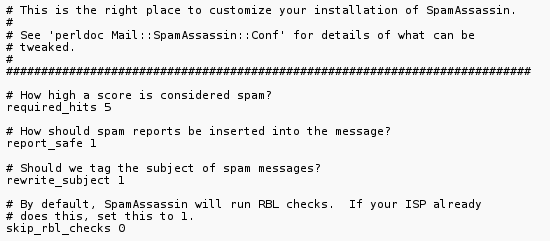
\includegraphics[width=\textwidth]{./annexes/local_sample.png}
 % local_sample.png: 0x0 pixel, 300dpi, 0.00x0.00 cm, bb=
 \caption{Exemple de configuration basique de SpamAssassin}
 \label{fig:local_sample}
\end{figure}


\subsubsection{Options de configuration}

Spam assassin possèdent plusieurs options dont certaine non activés par défaut. Il suffit de les ajouter aux fichiers 
de configuration.
Les options les plus importantes sont les suivantes:

\begin{description}
 \item [Désactiver les préférences utilisateurs]Dans \emph{/etc/default/spamassassin}, il faut changer la ligne d'options pour désactiver les préférences par utilisateur (qui serait normalement stockées dans leur home directory) et utiliser les préférences globales à la place. 
 \item [Options de score] \begin{description}
                           \item [required\_score n.nn (default:5)] Définit le score par défaut considérant un message comme SPAM. la valeur peut être un réel ou un entier
                           \item [score SYMBOLIC\_TEST\_NAME n.nn [ n.nn n.nn n.nn ]] Assigne les scores( voir ~\ref{score}) à un test donné.
                          \end{description}
\item 

\end{description}
\label{baye_conf}


\subsection{Les règles}

Il est possibles de définir des règles personnalisés. 

\section{ Utilisation }


SpamAssassin peut être utilisé avec des Mail Transfert Agent comme Postfix. On peut par exemple contrôler les messages
avec SpamAssassin juste après leurs reception par le demon SMTPD. Mais la façon la plus répandue est d'utiliser le MDA qui se charge
de filtrer satiquement les mails et de les déposer dans leurs boites mails respectives. 

\subsection{MDA}

Souvent couplé avec \emph{Postfix} (Le serveur de messagerie le plus utilisé dans le monde), procmail est le 
Mail Delivery Agent(Egalement connu comme Local Delivery Agent, sont des programmes qui sont responsable
de la délivrance des mails dans les boites des utilisateurs) que l'on trouve par défaut sur beaucoup de systèmes UNIX.
L'utilisation avec procmail est assez simple. Il faut modifier ou créer le fichier procmail.c qui se trouve dans le repertoire \emph{/etc.}.
Ainsi tout les messages passeront par SpamAssassin avant d'être délivéré par procmail. 
\linebreak
Un exemple de procmailrc minimale pour utiliser SPAM assassin:
\begin{lstlisting}[frame=single]  
DROPPRIVS=yes

LOGFILE=/var/log/procmail.log
VERBOSE=ON

# appel du deamon SpamAssassin
| /usr/bin/spamc -f

 :0e
{
   EXITCODE=$?
}
\end{lstlisting}
On peut tout à fait remplacer \emph{spamc} par \emph{spamassassin}. La seul différence étant au niveau des performances, 
chaque appel à la commande \emph{spamassassin}créant un processus distinct, alors que \emph{spamc} fait appel au demon \emph{spamd}.
A partir de là tout va passer à travers SpamAssassin.

\pagebreak

\subsection{SMTP}

Filtrer les mail à l'entré est aussi possible. 
        

\part{Autour de SpamAssasin}

\section{Comparatif avec des logiciels similaires à SpamAssassin}
Naturellement, il existe d'autres logiciels qui ont la même fonctionnalité que SpamAssassin, avec leur propres avantages et inconvénients, en voici quelques uns : \\
\\
\textbf{Spampal}
\begin{itemize}
\item Avantages : Peut être couplé à SpamAssassin, fonctionne de manière transparente en tant que proxy POP ou IMAP, utilise beaucoup de blacklists piochées sur le net pour filtrer le spam.

\item Inconvénients : SpamPal n'est pas totalement opérationnel au niveau du blocage par blacklist, et l'utilisation des blacklists DNS ralentissent et utilisent beaucoup de bande passante.
\end{itemize}

\textbf{K9}
\begin{itemize}
\item Avantages : Facile à mettre en place, léger.
\item Inconvénients : Ne gère pas le protocole IMAP ni le cryptage SSL.
\end{itemize}

\textbf{POPFile}
\begin{itemize}
\item Avantages : Très efficace une fois mis en place
\item Inconvénients : Compliqué à installer, ne gère pas les boites Hotmail
\end{itemize}

\textbf{Spamilihator}
\begin{itemize}
\item Avantages : Facile à installer, interface user-friendly
\item Inconvénients : Doit apprendre de beaucoup de Spams reçus avant d'être efficace
\end{itemize}

\textbf{Bogofilter}
\begin{itemize}
\item Avantages : Analyse très rapide des mails, temps d'apprentissage des Spams beaucoup plus court, très bon complement à SpamAssassin.
\item Inconvénients : Pas de réels inconvénients, Bogofilter reste le principal concurrent de SpamAssassin
\end{itemize}

\section{Quelques logiciels pouvant travailler avec SpamAssassin}
Les principaux logiciels avec lesquels SpamAssassin doit être couplé pour tirer profit du maximum de ses capacités sont évidemment les clients/serveurs de messagerie, comme par exemple :
\begin{itemize}
\item Postfix
\item Procmail
\item qmail
\item sendmail
\item Exim
\item Thunderbird
\item kmail
\item Evolution
\end{itemize}

Mais SpamAssassin peut aussi se coupler a d'autres logiciels anti-spam pour obtenir un meilleur résultat de filtrage. On peux notamment l'associer à SpamPal, mais le logiciel anti-spam auquel il est le plus souvent couplé est Bogofilter car il reste le concurrent le plus performant sur ce plan. Bien configurés, l'alliance des deux logiciels permet un filtrage quasi-optimal.
\end{document}

\section{Logiciel intégrant SpamAssin}

\section{modules}
